\section{EXAMPLES}\label{sec:examples}
As before, let $(X_n)_{n \geq 0}$ be the $N$-BRW governed by the point process $\scr{L}$ with logarithmic moment generating function $\psi$. In this section we provide some concrete examples and reflect upon how they fit into the previous sections' results. 







\subsection{Binary Gaussian N-BRW}\label{subsec:examples_gaussian_BRW}
Suppose that $\scr{L} = \delta_{Y_1} + \delta_{Y_2}$ where $Y_1, Y_2$ are i.i.d. normal with mean $\mu$ and variance $\sigma^2 > 0$. The logarithmic moment generating function takes the form
\begin{equation}\nonumber
\psi(t) = \log \Ex{e^{Y_1} + e^{Y_2}} = \mu t + \frac{\sigma^2 t^2}{2} + \log 2. 
\end{equation}
Clearly $\psi(t)$ is finite for all $t \in \R$, and solving for $t^* > 0$ in $\psi'(t^*) t^* = \psi(t^*)$ we get $t^* = \sqrt{\frac{2 \log 2}{\sigma^2}}$. Therefore $\scr{L}$ satisfies the hypothesis of Theorem \ref{thm:ExpTails_BrunDer_non_transformed}, and so 
\begin{equation}\nonumber
\lim\limits_{n \to \infty} \frac{\max X_n}{n} = v_N = \mu + \sqrt{\sigma^2 \log 4} - \frac{\pi^2 \sqrt{\sigma^2 \log 4}}{2 (\log N)^2} + o((\log N)^{-2}). 
\end{equation}
In fact, we could replace the Gaussian distribution with any distribution on $\R$ that has finite moment generating function on all of $\R$ and which puts less than $1/2$ mass on its essential supremum. The resulting point process would still satisfy the hypothesis of Theorem \ref{thm:ExpTails_BrunDer_non_transformed} by Proposition \ref{prop:jaffuel}. \\





\begin{figure}[!h]
\centering
\begin{minipage}{0.45\textwidth}
  \centering
  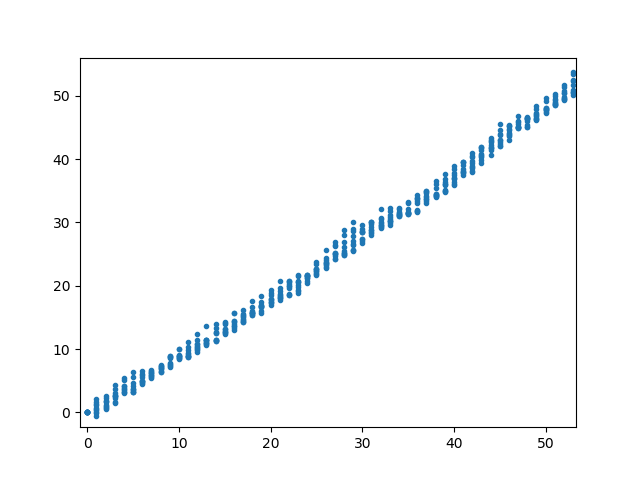
\includegraphics[width=.99\linewidth]{graphics/std_normal}
  \caption{Gaussian binary $N$-BRW with $N = 10$}
  \label{fig:normal}
\end{minipage}\hfill
\begin{minipage}{0.45\textwidth}
  \centering
  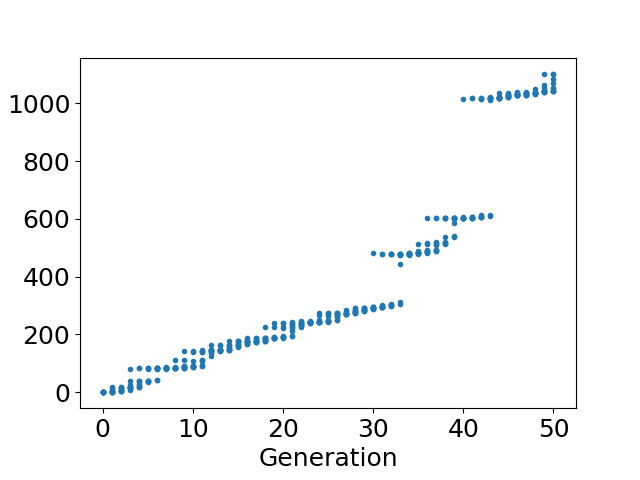
\includegraphics[width=.99\linewidth]{graphics/cauchy}
  \caption{Cauchy binary $N$-BRW with $N = 10$. }
  \label{fig:cauchy}
\end{minipage}\hfill%
\end{figure}






\subsection{Binary Bernoulli N-BRW}\label{subsec:binary_bernoulli_BRW}
Another natural choice might be $Y_1, Y_2$ i.i.d. Bernoulli with parameter $\alpha \in (0, 1)$. However, it turns out that the hypothesis of Theorem \ref{thm:ExpTails_BrunDer_non_transformed} is satisfied if and only if $\alpha \in (0, 1/2)$. This is because for $\alpha \geq 1/2$ the $Y_i$ put $\geq 1/2$ mass on their essential supremum (which in this case is equal to $1$) and the claim follows by Proposition \ref{prop:jaffuel}. \\

To confirm this consider the following. $\psi(t) = \log 2 + \log (\alpha e^t + 1 - \alpha)$ so if $f(t) \defeq t \psi'(t) - \psi(t)$ then $f'(t) = t \psi''(t) > 0$ for all $t > 0$. Now, as $f(0) = -\log 2 < 0$, the equation $f(t^*) = 0$ has a solution $t^* > 0$ if and only if $\lim_{t \to \infty} f(t) > 0$. We have
\begin{align*}
\lim\limits_{t \to \infty} f(t) &= \lim\limits_{t \to \infty} \left[\frac{\alpha t e^t}{\alpha e^t + 1 - \alpha} - \log(\alpha e^t + 1 - \alpha) - \log 2 \right] \\
								&= \lim\limits_{t \to \infty} \left[ t \big( 1 - \frac{1 - \alpha}{\alpha e^t + 1 - \alpha}\big) - t - \log (1 + \frac{1-\alpha}{\alpha} e^{-t}) - \log(2 \alpha) \right] \\
								&= - \log(2\alpha). 
\end{align*} 
Above expression is positive if and only if $\alpha \in (0, 1/2)$ as claimed. In \cite{exp_tails} Bérard and Gouéré note this as well and go on to show the following
\begin{theorem}[{{\cite[Theorems 4, 5]{exp_tails}}}]
For $\alpha = 1/2$ it holds that
\begin{equation}\nonumber
1 - v_N = \Theta(N^{-1})
\end{equation}
while for $\alpha \in (1/2, 1]$ we have
\begin{equation}\nonumber
- \log (1 - v_N) = \Theta(N). 
\end{equation}
\end{theorem}
\begin{remark}A slightly more general case of Bernoulli $N$-BRWs was studied by the authors \cite{couronne2014branching} using elementary methods, making it an accessible and enjoyable read. 
\end{remark}


\begin{figure}[!h]
\centering
\begin{minipage}{0.45\textwidth}
  \centering
  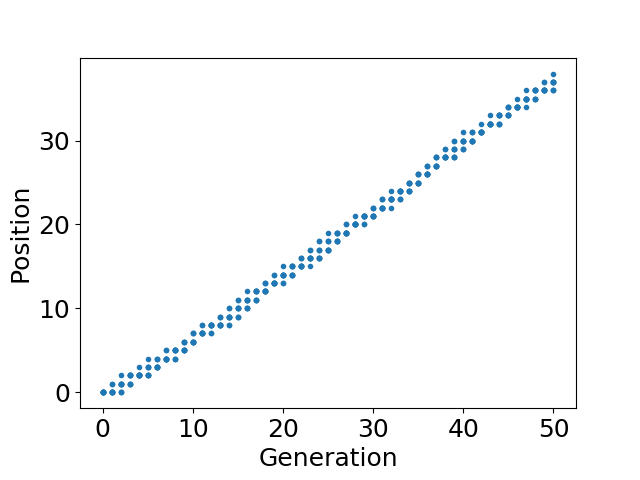
\includegraphics[width=.99\linewidth]{graphics/bernoulli_25}
  \caption{Bernoulli binary $N$-BRW with $N=10, p=0.25$. }
  \label{fig:ber25}
\end{minipage}\hfill
\begin{minipage}{0.45\textwidth}
  \centering
  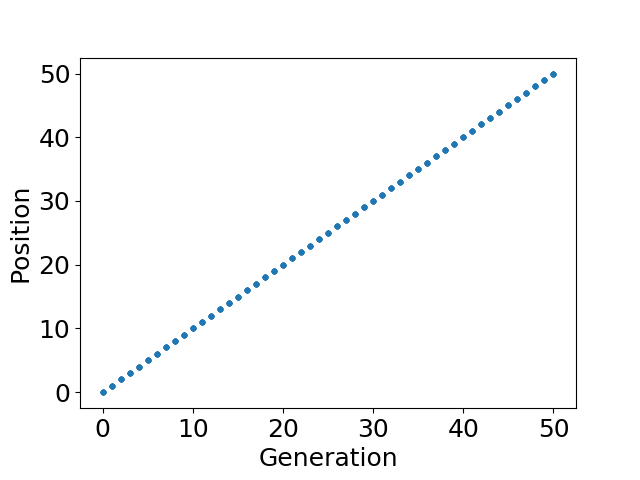
\includegraphics[width=.99\linewidth]{graphics/bernoulli_75}
  \caption{Bernoulli binary $N$-BRW with $N=10, p=0.75$. }
  \label{fig:ber75}
\end{minipage}\hfill%
\end{figure}




% \subsection{N-BBM}
% % Let $(B_t)_{t \geq 0}$ be a standard Branching Brownian Motion (as described in Section \ref{sec:examplessubsec:FKPP}) that branches at rate $\beta$ each time giving birth to $M$ particles. Standard BBM corresponds to the case $\beta = 1$ and $M = 2$. 
% Let $(B_t)_{t \geq 0}$ be a standard $N$-BBM (as described in Section \ref{subsec:FKPP}) started from $N\,\delta_0$. Clearly $(B_n)_{n \in \N}$ is an $N$-BRW, however explicitly describing its point process is not trivial. Nevertheless, its logarithmic moment generating function is easy to obtain. It is clear that $\# \scr{L}$ is distributed as the simple birth process $(M_t)_{t \geq 0}$ after one unit of time that is started from $M_0 = 1$ with escape rate equal to the number of particles alive. It is an elementary fact that $\E M_t = e^t$ so we get
% \begin{equation}
% \psi(t) = 1 + \frac{t^2}{2}. 
% \end{equation}
% Solving $\psi'(t^*) t^* = \psi(t^*)$ we obtain $t^* = \sqrt{2}$. By Theorem \ref{thm:ExpTails_BrunDer_non_transformed} we get
% \begin{equation}
% v_N \defeq \lim\limits_{n \to \infty} \frac{\max B_n}{n} = \sqrt{2} - \frac{\pi^2}{\sqrt{2}(\log N)^2} + o((\log N)^{-2})
% \end{equation}
% where the limit is both in $L^1$ and almost surely. We can use a simple sandwiching argument to get the corresponding result for continuous time. We have
% \begin{equation}\label{eqn:sandwich}
% \frac{\max B_t}{t} = \bigg( \frac{\max B_t - \max B_{\floor{t}}}{\floor{t}} + \underbrace{\frac{\max B_{\floor{t}}}{\floor{t}}}_{\to v_N\,a.s.\,\&\,L^1} \bigg) \underbrace{\frac{\floor{t}}{t}}_{\to 1}. 
% \end{equation}
% Fix $t \geq 0$ and let $\cal{P} \defeq (P_j)_{j \in [N]}$ be an i.i.d. collection of $\dPo{1}$ random variables. Further, let $\cal{Z} \defeq (Z^{j, k}_t)_{j \in \N,\,k \geq 1,\, t \geq 0}$ be a collection of i.i.d. standard Brownian motions independent of $\cal{N}$. There is an obvious coupling of $(B_s)_{\floor{t} \leq s < t}$ and the collections $\cal{P}$ and $\cal{Z}$. This coupling immediately yields the following upper bound: 
% \begin{equation}
% \max B_t - \max B_{\floor{t}} \stackrel{st.}{\leq} \sum\limits_{j=1}^N \sum\limits_{k=1}^{P_j} \sup\limits_{s \in [0, 1)} Z^{j, k}_s. 
% \end{equation}
% It is a well known fact that $\sup_{s \in [0, 1)} Z_s$ and $|Z_1| \in L^1$ have the same distribution for a standard Brownian motion $(Z_t)_{t \geq 0}$. In the same fashion we can obtain a lower bound and we find that
% \begin{equation}
% |\max B_t - \max B_{\floor{t}}| \stackrel{st.}{\leq} \cal{B}
% \end{equation}
% where the distribution of $\cal{B} \in L^1$ is independent of $t$. This gives $t^{-1} \max B_t \to v_N$ in $L^1$ while almost sure convergence follows by the Borel-Cantelli lemma. Indeed, let $(\cal{B}_j)_{j \geq 0}$ be an i.i.d. collection distributed like $\cal{B}$. Then
% \begin{equation}
% \Pr{t^{-1} \max B_t \nrightarrow v_N} \leq \sum\limits_{k = 1}^\infty \Pr{\cal{B}_n > n/k \text{ for infinitely many }n \in \N} = 0, 
% \end{equation}
% since $\int_0^\infty \Pr{\cal{B} > \lambda} d\lambda = \E\cal{B} < \infty$. 


% Clearly by the Markov property, for any $t \geq 0$ we have
% \begin{equation}
%  \max B_t - \max B_{\floor{t}} \leq \sup\limits_{s \in [0, 1)} \left[ \max B_{\floor{t} + s} - \max B_{\floor{t}} \right] \stackrel{st.}{\leq} \sup\limits_{s \in [0, 1)} \max B_s. 
% \end{equation}

% This


% \begin{equation}
% \scr{L} = \sum\limits^P_{j=1} \delta_{Y_j}, 
% \end{equation}
% where $P \sim 1 + \dPo{\beta}$ and $Y_j \sim \dNorn{0, 1}$ for $j = 1, 2, ...$ are all independent. By a simple calculation
% \begin{equation}
% \psi(t) = \log
% \end{equation}


\subsection{N-BRW with Cauchy spine}
Consider the model where $\scr{L}$ is given by a Poisson Point Process (PPP) with intensity measure $e^{-x} \nu_\alpha (dx)$ where $\nu_\alpha$ is some $\alpha$-stable distribution with $\nu_\alpha(0, \infty) \in (0, 1)$. By The Slivnyak-Mecke Theorem \cite[Theorem 1.13]{baccelli2009stochastic} we have
\begin{equation}\nonumber
\E \sum\limits_{l \in \scr{L}} e^l = \int_\R e^\lambda e^{-\lambda} \nu_\alpha(d\lambda) = 1
\end{equation}
so $\scr{L}$ satisfies (\ref{eqn:BRW_V_Ass}). We claim that the spine is in the domain of attraction of $\nu_\alpha$. Indeed, we just have to observe that 
\begin{equation}\nonumber
\Pr{X \leq x} \defeq \E \sum\limits_{l \in \scr{L}} \Ind_{\{ l \leq x \}} e^l  = \int\limits^x_{-\infty} \nu_\alpha(d \lambda), 
\end{equation}
 by the Slivnyak-Mecke theorem. Since stable distributions are in their own domains of attraction (\cite[p. 576]{feller1957introduction}) we are done. 

\begin{remark}
In Figure \ref{fig:Cauchy_spine} we see a simulation of the above model. Producing the image was not entirely straightforward: the PPP with intensity $p_\alpha (dx) = e^{-x} \nu_\alpha (dx)$ has almost surely infinitely many points on the negative real line. Thus we cannot generate the entirety of the Cauchy PPP - it is enough to generate the rightmost $N$ points. To do so we had to make use of multiple properties of PPPs: if $A, B \subset \R$ are disjoint then the number and position of points in $A, B$ are independent. Furthermore the number of points in $A$ is a Poisson random variable with mean $\int_A p_\alpha(dx)$ conditional on which the position of points is i.i.d. with unnormalised density $p_\alpha$ on $A$. To make simulations reasonably fast we also had to make use of the fact that PPPs are additive and that $e^{-x}/(1+x^2)$ can be integrated in closed form.  
\end{remark}

\begin{figure}[!h]
  \centering
  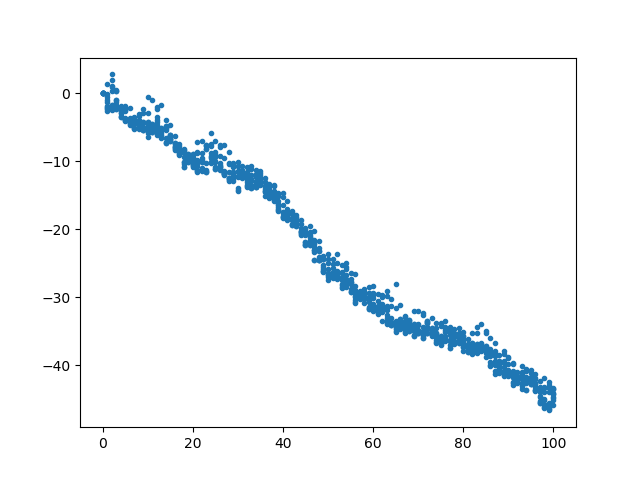
\includegraphics[width=.99\linewidth]{graphics/cauchy_PPP}
  \caption{$N$-BRW with Cauchy spine. }
  \label{fig:Cauchy_spine}
\end{figure}


\subsection{Binary N-BRW with polynomial tails}
As in Sections \ref{subsec:examples_gaussian_BRW} and \ref{subsec:binary_bernoulli_BRW}, let $\scr{L} = \delta_{Y_1} + \delta_{Y_2}$ where this time $Y_1, Y_2$ are i.i.d. with distribution given by
\begin{equation}\nonumber
\Pr{Y_1 > x} = \frac{1}{x^\alpha},\qquad\forall\,x \geq 1
\end{equation}
for some $\alpha > 0$. If $\alpha > 1$ we can use the notation of Section \ref{sec:poly_result} to get $c_N = (2N \log_2 N)^{1/\alpha}$ so that
\begin{equation}\nonumber
v_N \sim \frac{\rho_\alpha c_N}{\log_2 N} \propto \left( \frac{N}{(\log N)^{\alpha - 1 }} \right)^{1/\alpha}
\end{equation}
by Theorem \ref{thm:poly_tails_result}. For $\alpha = 1$ we are in case $(c)$ of Theorem \ref{thm:poly_tails_result} and we have $c_N = 2 N \log_2 N$ and $b_N = \int^n_1 dx/x = \log n + \cal{O}(1)$. Thus loosely speaking we get 
\begin{equation}\nonumber
\frac{\max X_n}{n \log n} \approx \delta_{2N}. 
\end{equation}
It is worth noting that in both of these cases the behaviour of the system is vastly different from the Brunet-Derrida behaviour. In particular, the speed at which the particles propagate diverges as $N \to \infty$. 
\newpage
